\chapter{Índices espectrales}

El objetivo de esta clase es generar e interpretar índices espectrales, utilizando una imagen \emph Sentinel-2.


\section{NDVI}
El NDVI \emph{(Normalized Difference Vegetation Index)} es uno de los índices de uso más extendido en teledetección. Utiliza la diferencia entre la absorción de la clorofila en el rojo y la reflectancia del infrarrojo cercano, que se relaciona con la biomasa fotosintéticamente activa.

Para calcularlo, seleccione:

\begin{center}
\menu{Optical>Tematic Land Processing > Vegetation Radiometric Indices>NDVI Processor}
\end{center}

Se desplegará una nueva ventana (Figura \ref{fig:NDVI}). En \menu{Directory} seleccione la carpeta de salida para guardar el archivo en formato BEAM-DIMAP. Presione \menu {Run} para finalizar. El producto \emph{NDVI} se cargará en el \menu{Product Explorer}. Para visualizarlo realice doble click sobre el producto recién creado y seleccione \emph{ndvi}. En el visualizador se desplegará la imagen obtenida en escala de grises.

\begin{figure}[h!]
    \centering
    \subfloat[1-I/O Parameters]{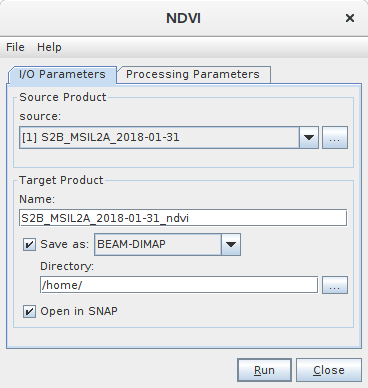
\includegraphics[width=0.4\textwidth]{fig:NDVI.png}\label{fig:NDVI-impar}}
    \hspace{1cm}
    \subfloat[Processing parameters]{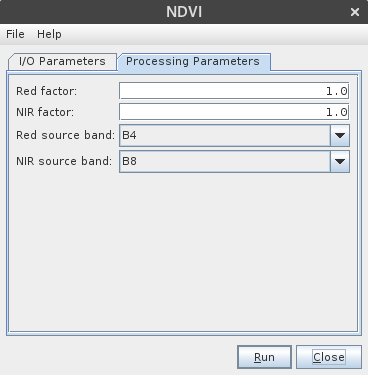
\includegraphics[width=0.4\textwidth]{fig:NDVI-par.png}\label{fig:NDVI-par}}
    \caption{Generación del \emph{NDVI}.}
    \label{fig:NDVI}
\end{figure}

Identifique los diferentes usos y coberturas en el producto NDVI. Visualice un parche homogeneo de una cobertura y posicione el cursor sobre un pixel. Obtenga el valor de NDVI utilizando la herramienta  \menu {pixel info}. Recorra la imagen con el cursor y observe los valores que toma el \emph{NDVI} para cada cobertura. Relacione los valores con la escala de grises de la imagen.


\section{NDWI}

El NDWI \emph{(Normalized Difference Water Index)} es un estimador del contenido de agua en el canopeo vegetal que interactua con la radación solar incidente. Puede ser utilizado de manera complementaria al NDVI para monitorear el estado fisiológico de la vegetación. Sin embargo, es sensible al ruido que produce el suelo sin cobertura.


En este caso se utilizará una herramienta que permite realizar operaciones matemáticas. Seleccione \menu{Raster>Band maths...} (Figura \ref{fig:bm2}).

 \begin{figure}[h!]
     \centering
     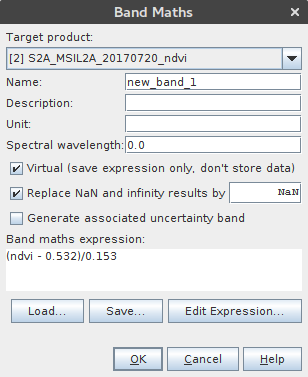
\includegraphics[width=0.4\textwidth]{fig:bm.png}
     \caption{Álgebra de bandas.}
     \label{fig:bm2}
 \end{figure}


En el casillero \emph{Band math expression} deberá escribir la expresión matemática utilizando el nombre de las bandas y los correspondientes operadores. En este caso:

\begin{center}
\texttt{(B11-B8)/(B11+B8)}
\end{center}

En la opción \emph{Name} escriba ndwi, para asignarle un nombre a la nueva banda creada y presione \emph{OK}, para finalizar.

 {\bf Importante:} Por defecto se crea una banda virtual que calcula los valores \emph{al vuelo}. Para forzar el cálculo de la banda destilde la opción \emph{Virtual}.

El producto \emph{NDWI} se cargará en \menu{Product Explorer}. Para visualizarlo realice doble click sobre \menu {S2B\_MSIL2A\_2018-01-31>Bands} y seleccione \emph{ndwi}. Se desplegará la imagen en escala de grises. Compare y analice tal como lo hizo con el NDVI.

\section{SAVI}

El SAVI \emph{(Soil Adjusted Vegetation Index)}, al igual que el NDVI utiliza la diferencia entre la absorción de la clorofila en el rojo y la reflectancia del infrarrojo cercano, con la ventaja de reducir el error que aporta la reflectancia del suelo, ajustandolo según el tipo de sustrato y porcentaje de cobertura.

Para calcularlo, seleccione

\begin{center}
\menu{Optical>Tematic Land Processing > Vegetation Radiometric Indices>SAVI Processor}.
\end{center}

Se desplegará una nueva ventana (Figura \ref{fig:NDVI}). En \menu{Directory} seleccione la carpeta de salida para guardar el archivo en formato BEAM-DIMAP. Para finalizar presione \menu {Run}. El producto \emph{SAVI} se cargará en \menu{Product Explorer}. Para visualizarlo realice doble click sobre \menu {S2B\_MSIL2A\_2018-01-31>Bands} y seleccione \emph{savi}. Se desplegará la imagen en escala de grises. Compare y analice tal como lo hizo con el NDVI.

\section{Visualización con paleta de colores}

Una forma práctica de visualizar productos monobanda como el NDVI o SAVI es utilizando una paleta de colores, donde los valores bajos, intermedios y altos se muestren en forma de gradiente.

Despliegue el producto NDVI. En \menu {Colour manipulation} podrá ver la distribución estadística de los pixeles (Figura \ref{fig:color-man}). Seleccione la función \menu{import color palette from text file}, allí encontrará disponibles varias paletas de colores, seleccione \directory{meris\_veg\_index}. Se abrirá una pequeña ventana en la que figura la siguiente pregunta: \emph{Automatically distribuite points of colour palette between min/max?}, presione \menu{Yes}.

La imagen aparecerá en tonos de verde, amarillo, naranja y marrón. Los valores NDVI altos se visualizarán en verde, los intermedios en amarillo y los valores bajos en marrón oscuro. Analice la relación entre los valores de los pixeles y los colores observados (Figura \ref{fig:color-man-meris}).

Realice el mismo procedimiento para el SAVI.

\begin{figure}[h!]
    \centering
    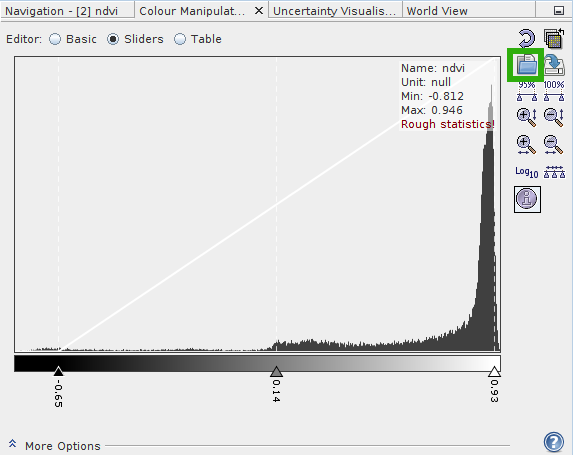
\includegraphics[width=0.6\textwidth]{fig:colour-man.png}
    \caption{Herramienta de Manipulación de Color. En la opción Sliders se observa la distribución estadística de valores de NDVI. El recuadro verde marca el \menu{import color palette from text file}}
    \label{fig:color-man}
\end{figure}

\begin{figure}[h!]
    \centering
    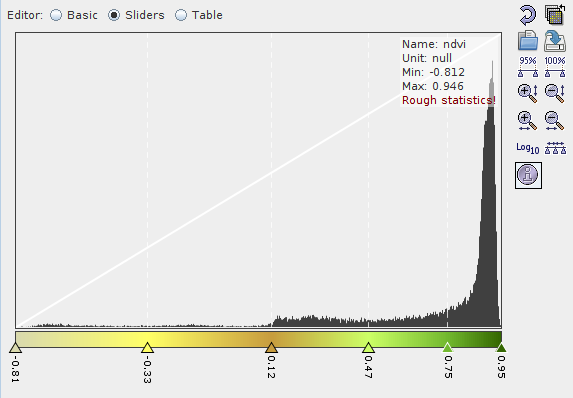
\includegraphics[width=0.6\textwidth]{fig:colour-man-meris.png}
    \caption{Herramienta de Manipulación de Color. En Sliders se observa la distribución estadística de valores de NDVI para la paleta de color meris.}
    \label{fig:color-man-meris}
\end{figure}

\section{Cálculo de estadísticas zonales}

En la práctica es bastante común calcular las estadísticas básicas de un conjunto de pixeles de una misma cobertura, en lugar de observar un valor único. El procedimiento requiere varios pasos ya que es indispensable primero crear los polígonos de parches homogéneos, sobre los cuales se obtendrán los estadísticos.
\subsection{Creación de vectores}

	En primer lugar se deberán crear los contenedores vectoriales. Para ello, seleccione \menu{Vector>New Vector Data Container}, coloque Selva paranaense como nombre del vector y presione \menu{OK} (Figura \ref{fig:vector-container}). Luego, usando  \menu {Polygon Drawing Tool} (Figura \ref{fig:drawing}), deberá dibujar el polígono sobre un parche homogéneo de la cobertura.

  Una vez que selecciona la herramienta, haga click sobre la imagen y se abrirá la ventana \menu{Select vector data container}, elija en éste caso Selva paranaense y dibuje el vector. Sobre la imagen, haga un click por cada vértice que considere necesario y finalice el polígono con doble click. Puede crear varias geometrías dentro de un mismo contenedor. Repita este paso para todas las coberturas observadas.

  \begin{figure}[h!]
      \centering
      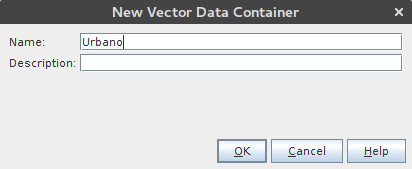
\includegraphics[width=0.4\textwidth]{fig:vector-cont.png}
      \caption{Herramienta Vector Container}
      \label{fig:vector-container}
  \end{figure}


  \begin{figure}[H]
      \centering
      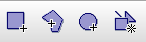
\includegraphics[scale=0.4]{fig:drawing.png}
      \caption{Herramientas para generar poligonos.}
      \label{fig:drawing}
  \end{figure}

\subsection{Cálculo de estadísticos}

	Seleccione \menu{Analisis>Statistics} y se abrirá una nueva ventan (Figura \ref{fig:estadistica-b}). Tilde la opción \menu{Use ROI mask(s)} para que se habilite la lista de vectores creados anteriormente. Elija el vector deseado y presione \menu{Refresh view}.


\begin{figure}[h!]
    \centering
    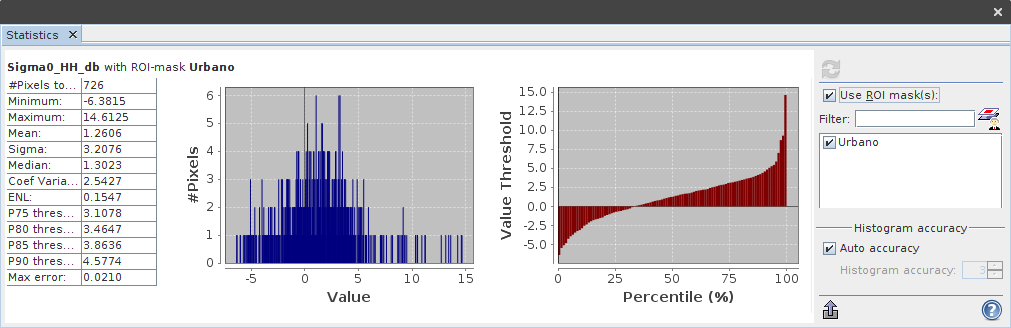
\includegraphics[width=0.8\textwidth]{fig:estadistica.png}
    \caption{Cálculo de estadísticas en un polígono.}
    \label{fig:estadistica-b}
\end{figure}


\section{Actividad práctica}

Visualice las imágenes de NDVI, NDWI y SAVI con la paleta de color \directory{meris\_veg\_index}. Identifique:

  \begin{itemize}
  \item Selva paranaense
  \item Cultivo
  \item Suelo sin cobertura vegetal
  \item Agua del embalse Urugua-í
  \end{itemize}

Con la herramienta \menu{pixel info} obtenga el valor del pixel de cada cobertura en las tres imágenes y realice un cuadro comparativo.

\begin{enumerate}
\item Para el producto NDVI ¿Qué cobertura tiene mayor valor? ¿Qué cobertura tiene menor valor? ¿Qué significan los valores negativos?
\item Grafique las firmas espectrales para cada cobertura y analice cual es la relació n entre las bandas del Rojo e Infrarrojo cercano.
\item Para el producto NDWI ¿Qué cobertura tiene mayor valor? ¿Qué cobertura tiene menor valor? Compare con los valores de NDVI, ¿Qué ocurre y a qué se debe?
\item Para el producto SAVI ¿Qué cobertura tiene mayor valor? ¿Qué cobertura tiene menor valor? Compare con los valores de NDVI, ¿Qué ocurre y a qué se debe?

\end{enumerate}



Estas preguntas y actividades no serán evaluadas. Su objetivo es discutirlas en el foro de consultas e intercambio de la clase.

%Comparar NDVI entre coberturas
%Comparar NDWI entre coberturas
%Comparar SAVI o GEMI
% Comparar la relacioon GEMI vs NDVI
% Hacer tabla comparativa entre indices


%Ver cómo manejar el tema de borrar pines en las comparaciones
% Añadir al anexo las longitudes de onda x mision satelital.
